\begin{center}\rule{0.5\linewidth}{0.5pt}\end{center}

\hypertarget{gpioux53e3ux7684ux5f15ux811aux987aux5e8f}{%
\subsection{GPIO口的引脚顺序}\label{gpioux53e3ux7684ux5f15ux811aux987aux5e8f}}

如图,单号引脚和双号引脚分别在一排。 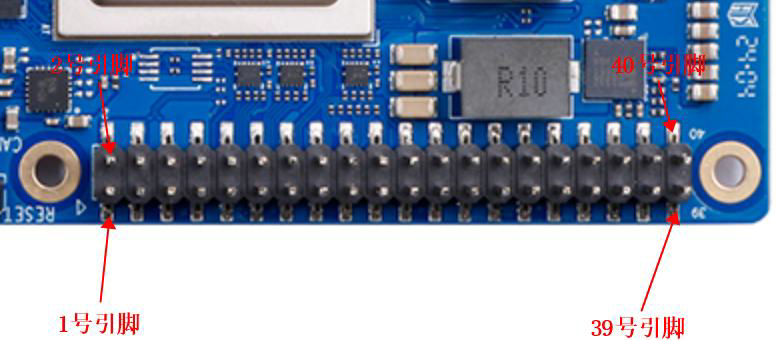
\includegraphics{img2/gpio.png}
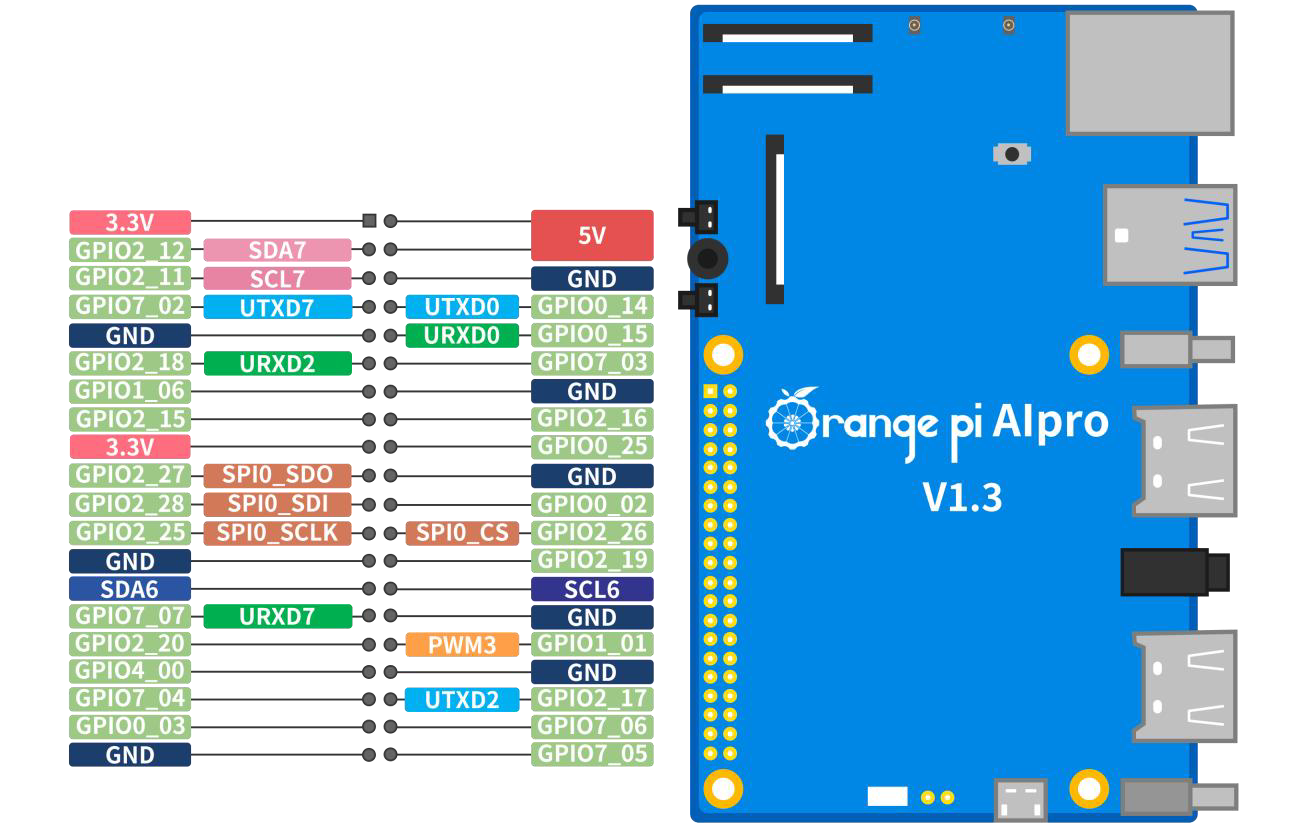
\includegraphics{img2/gpio2.png}

注意事项: 1. 40 pin 接口中总共有26 个GPIO 口,但8 号和10
号引脚默认是用于调试串 口功能的,并且这两个引脚和Micro USB
调试串口是连接在一起的,所以这两个 引脚请不要设置为GPIO 等功能。 2.
所有的GPIO 口的电压都是3.3v。 3. 40 pin 接口中27 号和28 号引脚只有I2C
的功能,没有GPIO 等其他复用功 能,另外这两个引脚的电压默认都为1.8v。
